\documentclass[
size=10pt,
paper=screen,
mode=present,
display=slidesnotes,
style=mc,
nohandoutpagebreaks,
%pauseslide,
fleqn,
clock,
,draft
]{powerdot}

\input{tex/common}

\pdsetup{
  lf = Tomasz Golan,
  cf = MC generators @ NuSTEC
}

\title{What is inside MC generators... \\ {\LARGE ...and why it is wrong}}
\author{Tomasz Golan}
\date{NuSTEC, Okayama 2015}

\begin{document}

\maketitle

%\section{Monte Carlo method}

%\begin{wideslide}{Buffon's needle problem}
\null\vfill

  \twocolumn
  {
    {\it Suppose we have a floor made of parallel strips of wood, each the same width, and we drop a needle onto the floor. What is the probability that the needle will lie across a line between two strips?}
    
    \sep
    
    {\it\hfill Georges-Louis Leclerc,\\\hfill Comte de Buffon\\\hfill 18th century}
  }
  {
    \sep\sep
    \centering\input{figures/buffon.tex}
  }
  
  \vspace{-10pt}
  \myBoxFullWidth{Monte Carlo without computers}
  
  \twocolumn
  {
    If needle length ($l$) $<$ lines width ($t$):
    
    $$P = \frac{2l}{t\pi}$$
    
    which can be used to estimate $\pi$:
    
    $$\pi = \frac{2l}{tP}$$
  }
  {
    MC experiment was performed by Mario Lazzarini in 1901 by throwing 3408 needles:
    
    $$\pi = \frac{2l \cdot 3408}{t \cdot \#red} = \frac{355}{113} = 3.14159292$$
  }
  
\vfill\null
\end{wideslide}

\begin{wideslide}[toc = From Solitaire to MC]{From Solitaire to Monte Carlo method}
\null\vfill

    \twocolumn
    {
      \begin{itemize}
	\item Stanis{\l}aw Ulam was a Polish mathematician
	\item He invented the Monte Carlo method while playing solitaire
	\item The method was used in Los Alamos, performed by ENIAC computer
      \end{itemize}  
      
      \includegraphics[width=\columnwidth]{figures/eniac1946.eps}
    }
    {
      \includegraphics[width=\columnwidth]{figures/solitaire.eps}
      \begin{itemize}
	\item What is a probability of success in solitaire?
	\begin{itemize}
	  \item Too complex for an analytical calculations
	  \item Lets try $N = 100$ times and count wins
	  \item With $N \rightarrow \infty$ we are getting closer to correct result
	\end{itemize}
      \end{itemize}
    }
 
\vfill\null
\end{wideslide}

\begin{slide}{Newton-Pepys problem}
\null\vfill

  \twocolumn
  {
    {\it
    Which of the following three propositions has the greatest chance of success?
    
    \begin{itemize}
      \item[A] Six fair dice are tossed independently and at least one “6” appears.
      \item[B] Twelve fair dice are tossed independently and at least two “6”s appear.
      \item[C] Eighteen fair dice are tossed independently and at least three “6”s appear.
    \end{itemize}
    }
  }
  {
    \sep\sep\sep\sep
    \centering\scalebox{0.15}{\input{figures/dice.tex}}
  }

\vfill\null
\end{slide}

\begin{slide}[toc=]{Newton-Pepys problem: analytical attempt}
\null\vfill

  \begin{itemize}
    \item First, lets go back to high school and calculate this analytically
    \item Let $p = \frac{1}{6}$ be the probability of rolling $6$
    \item The probability of not rolling $6$ is $(1 - p)$
    
    \item[A] six attempts, at least one six

    $$P_A = 1 - (1 - p)^6 \approx 0.6651$$

    \vspace{-5pt}
    \item[B] twelve attempts, at least two sixes
    
    $$P_B = 1 - (1 - p)^{12} - {12 \choose 1}p(1 - p)^{11} \approx 0.6187$$

    \vspace{-5pt}
    \item[C] eighteen attempts, at least three sixes
    
    $$P_C = 1 - (1 - p)^{18} - {18 \choose 1}p(1 - p)^{17} - {18 \choose 2}p^2(1 - p)^{16} \approx 0.5973$$
  
  \end{itemize}

\vfill\null
\end{slide}

\begin{wideslide}[method=direct,toc=]{Newton-Pepys problem: MC attempt}
\null\vfill

  \begin{minipage}{0.45\textwidth}
    \begin{itemize}
     \item MC attempt is just ``performing the experiment'', so we will be rolling dices
     \item Roll $6n$ times and check if number of sixes is greater or equal $n$
     \item Repeat $N$ times and your probability is given by:
     
     $$P = \frac{\mbox{number of successes}}{N}$$
    \end{itemize}
  \end{minipage}\hspace{0.05\textwidth}\begin{minipage}{0.5\textwidth}
{\small
\begin{verbatim}
def throw (nSixes):
  n = 0
  for _ in range (6 * nSixes):
    if random.randint (1, 6) == 6: n += 1
  return n >= nSixes
  
def MC (nSixes, nAttempts):
  n = 0
  for _ in range (nAttempts):
    n += throw (nSixes)
  return float (n) / nAttempts

if __name__ == "__main__":
  for i in range (1, 4):
    print MC (i, 1000)
\end{verbatim}
}
  \end{minipage}
  
\vfill\null
\end{wideslide}

\begin{slide}[toc=]{Newton-Pepys problem: summary}
\null\vfill

  \begin{itemize}
    \item Your MC result depends on $N$
    \item Results for $N = 100$:
    
    \begin{eqnarray*}
      P_A & = & 0.71, 0.68, 0.76, 0.65, 0.68 \hspace{20pt}{\color{pdcolor3}P_A^{true} = 0.6651} \\
      P_B & = & 0.70, 0.56, 0.60, 0.63, 0.69 \hspace{20pt}{\color{pdcolor3}P_B^{true} = 0.6187}\\
      P_C & = & 0.62, 0.62, 0.53, 0.57, 0.62 \hspace{20pt}{\color{pdcolor3}P_C^{true} = 0.5973}
    \end{eqnarray*}
    
    \item Results for $N = 10^6$:
    
    \begin{eqnarray*}
      P_A & = & 0.6655, 0.6648, 0.6653, 0.6662, 0.6653 \\
      P_B & = & 0.6188, 0.6191, 0.6191, 0.6190, 0.6182 \\
      P_C & = & 0.5975, 0.5979, 0.5972, 0.5978, 0.5973
    \end{eqnarray*}
    
    \item Your MC results also depends on the way how random numbers were generated
    
  \end{itemize}

\vfill\null
\end{slide}

%\begin{wideslide}[toc = Simple Monte Carlo, method=direct]{Simple Monte Carlo - coin flipping}
%\null\vfill
%
%  \begin{itemize}
%    \item What is the probability of getting head / tail when throwing a coin?
%  \end{itemize}
%  
%  \begin{minipage}{0.7\textwidth}
%  \begin{itemize}
%    \item One can use MC method to calculate this:
%    \begin{itemize}
%      \item get $N$ times a random number $x \in \{0,1\}$
%      \item check how many ($n$) times $x = 1$
%      \item $P = \frac{n}{N}$
%    \end{itemize}
%    \item One-line example in Python:
%  \end{itemize}
%  \end{minipage}\begin{minipage}{0.3\textwidth}
%		  
\includegraphics[width=0.5\columnwidth]{figures/coin.eps}
%                \end{minipage}
%
%  {\small\color{pdcolor3}
%  \begin{verbatim}
%MC = lambda N: len(filter(lambda x: random.randint(0,1), range(N))) / float(N)     
%  \end{verbatim}
%  }
%  \begin{minipage}{0.55\textwidth}
%  \begin{itemize}
%   \item If you do not like one-liners:
%  \end{itemize}
%  \vspace{-20pt}  
%  {\small\color{pdcolor3}
%  \begin{verbatim}
%def MonteCarlo(N):
%  n = 0
%  for _ in range(N):
%    if random.randint(0,1): n += 1
%  return float(n) / N   
%  \end{verbatim}
%  }
%  \end{minipage}\begin{minipage}{0.45\textwidth}
%		  \vspace{-10pt}
%		  \begin{itemize}
%		   \item Some results for MC(100):
%		   \item[]
%		   0.51, 0.48, 0.61, 0.46, 0.57, 0.46
%		   \item Some results for MC(100000):
%		   \item[]
%		   0.50139, 0.49798, 0.49933, 0.5005
%		  \end{itemize}
%                \end{minipage}
%
%\vfill\null
%\end{wideslide}

%\begin{slide}[toc=PRNG]{Pseudorandom number generator}
\null\vfill

  \begin{itemize}
    \item PRNG is an algorithm for generating a sequence of ``random'' numbers
    \item Example: middle-square method (used in ENIAC)
    \begin{itemize}
      \item take $n$-digit number as your seed
      \item square it to get $2n$-digit number (add leading zeroes if necessary)
      \item $n$ middle digits are the result and the seed for next number
    \end{itemize}
    \item Middle-square method for $n = 4$ and base seed = $1111$:
  \end{itemize}
  \vspace{-10pt}
  \begin{eqnarray*}
    1111^2 & = & {\color{pdcolor3}01}2343{\color{pdcolor3}21} \rightarrow 2343 \\
    2343^2 & = & {\color{pdcolor3}05}4896{\color{pdcolor3}49} \rightarrow 4896 \\
    & \vdots & \\
    1111^2 & = & {\color{pdcolor3}01}2343{\color{pdcolor3}21} \rightarrow 2343 
  \end{eqnarray*}
    
\vfill\null
\end{slide}

\begin{slide}[toc=]{Pseudorandom number generator}
\null\vfill

  \begin{itemize}
    \item Nowadays, more sophisticated PRNGs exist, but they also suffer on some common problems:
    \begin{itemize}
      \item periodicity / different periodicity for different base seed
      \item nonuniformity of number distributions
      \item correlation of successive numbers
    \end{itemize}
  \end{itemize}

  \twocolumn
  {
    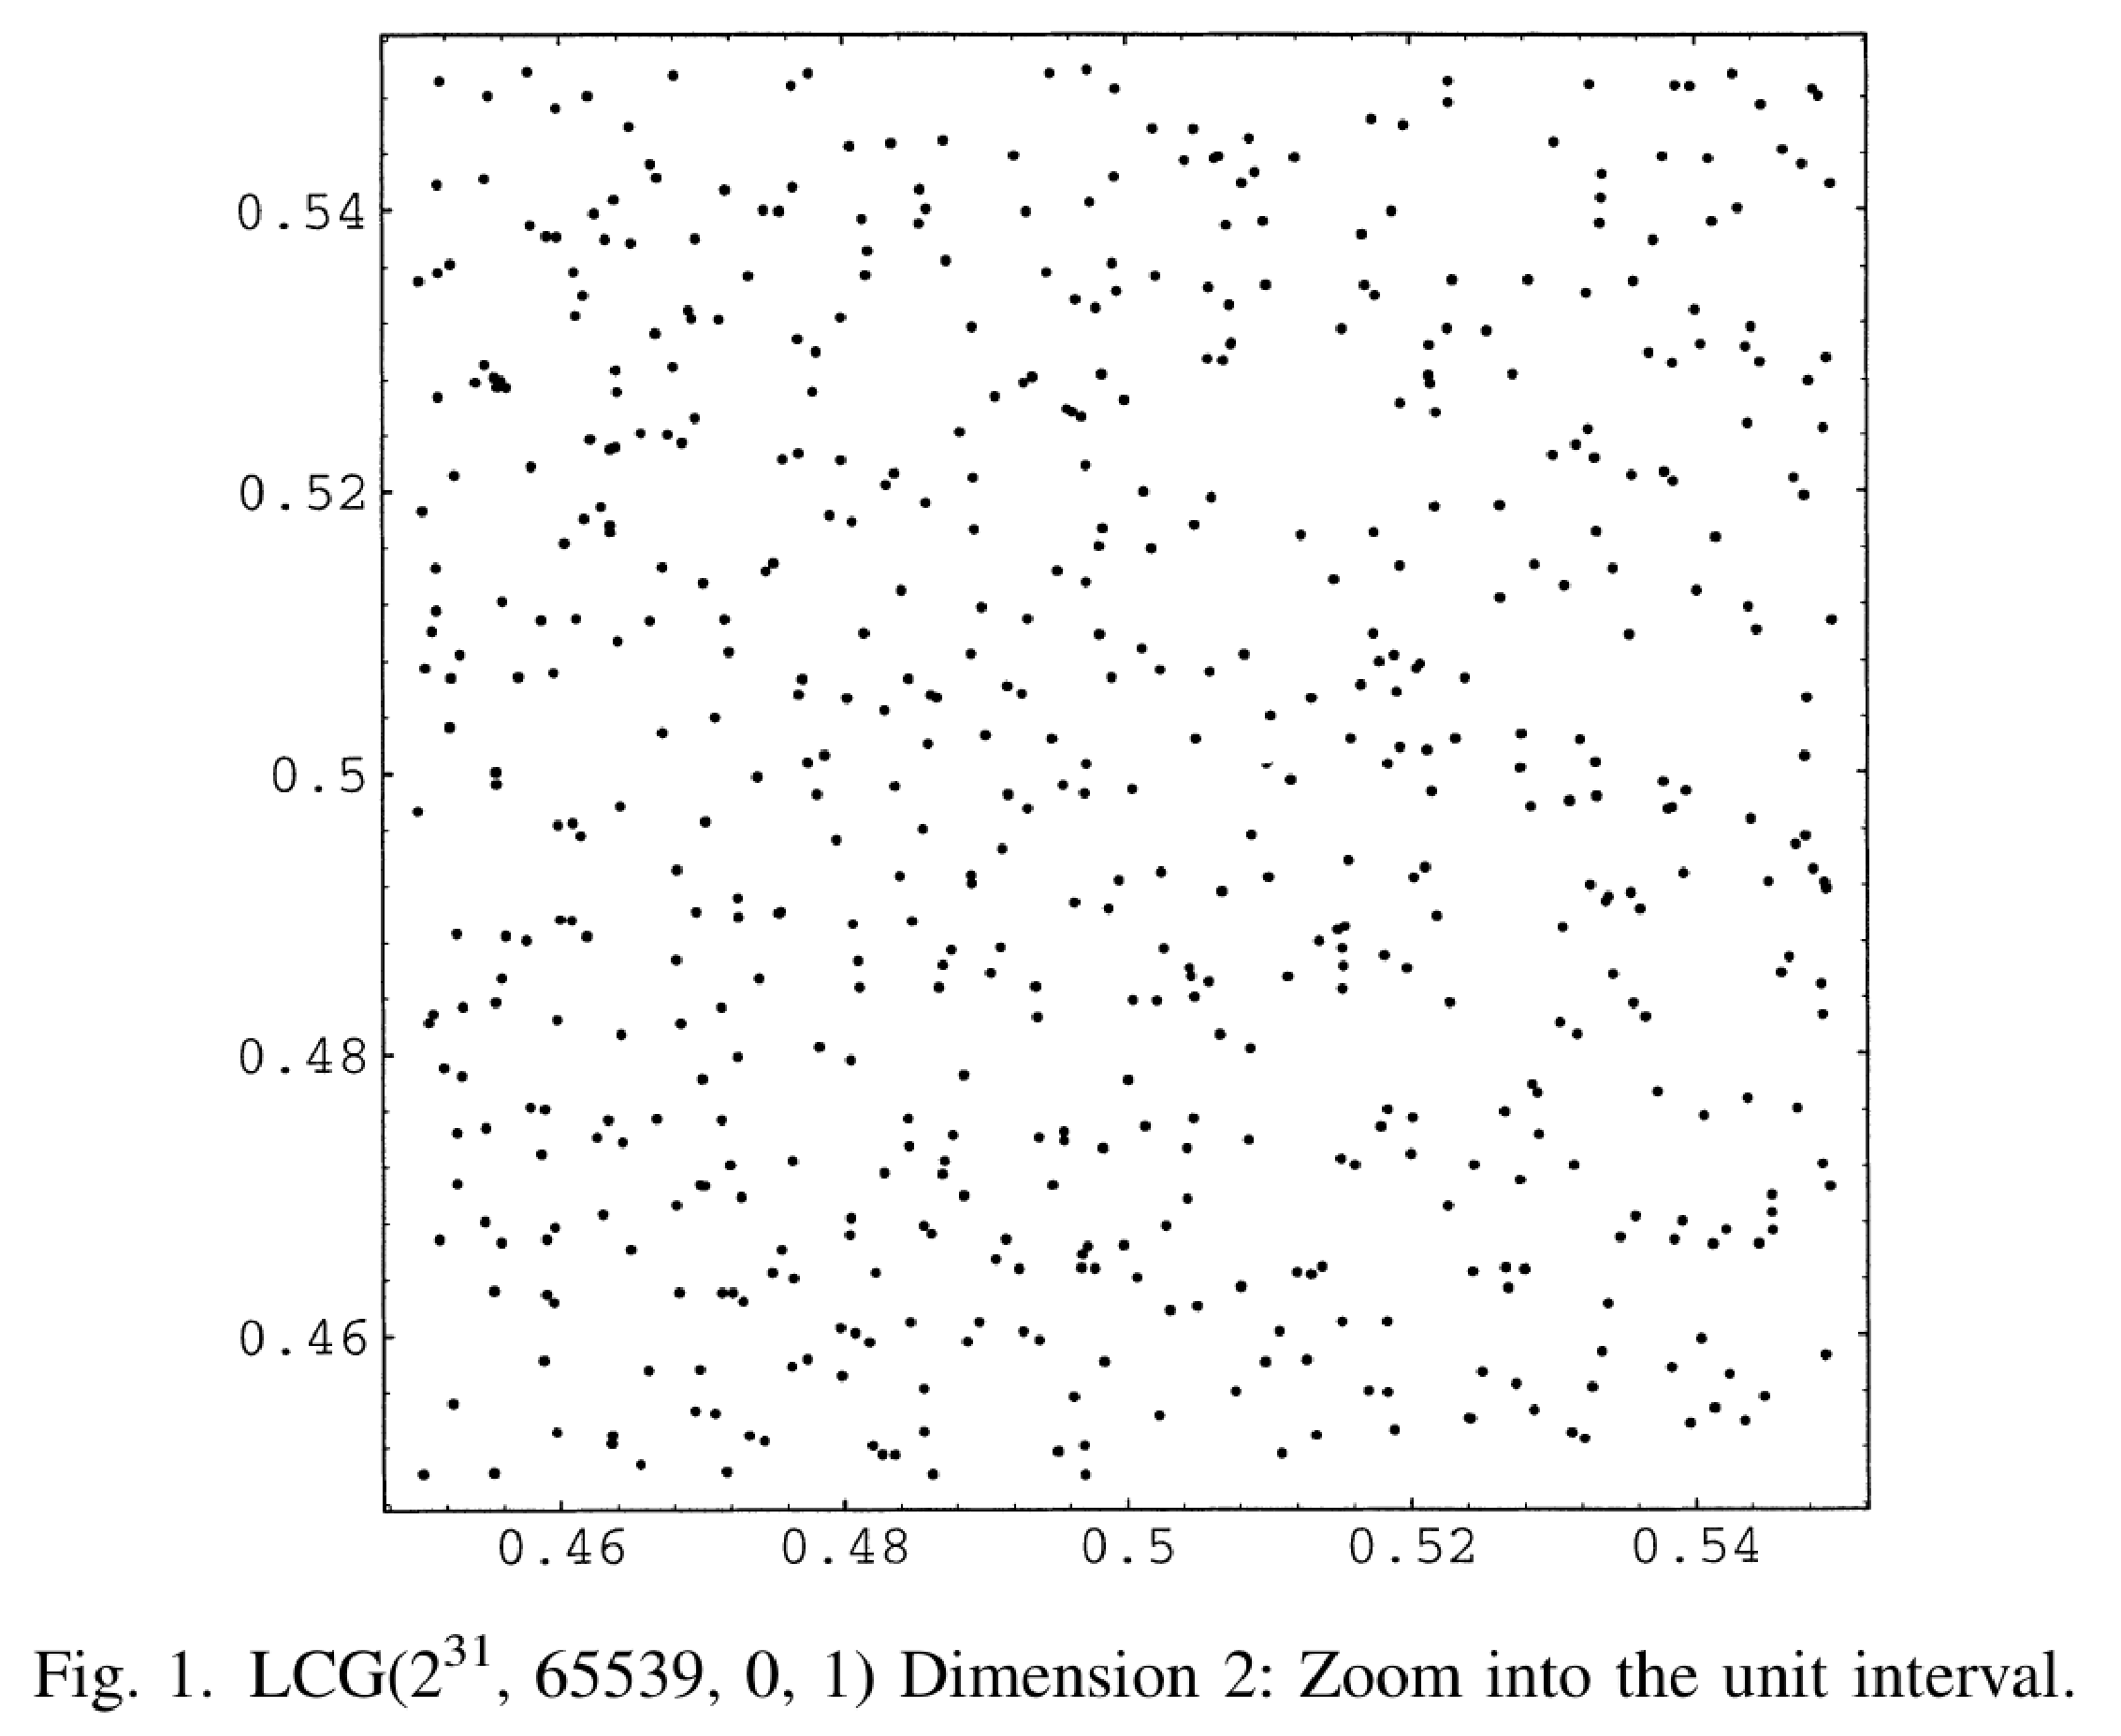
\includegraphics[width=\columnwidth]{figures/random2d.eps}
  }
  {
    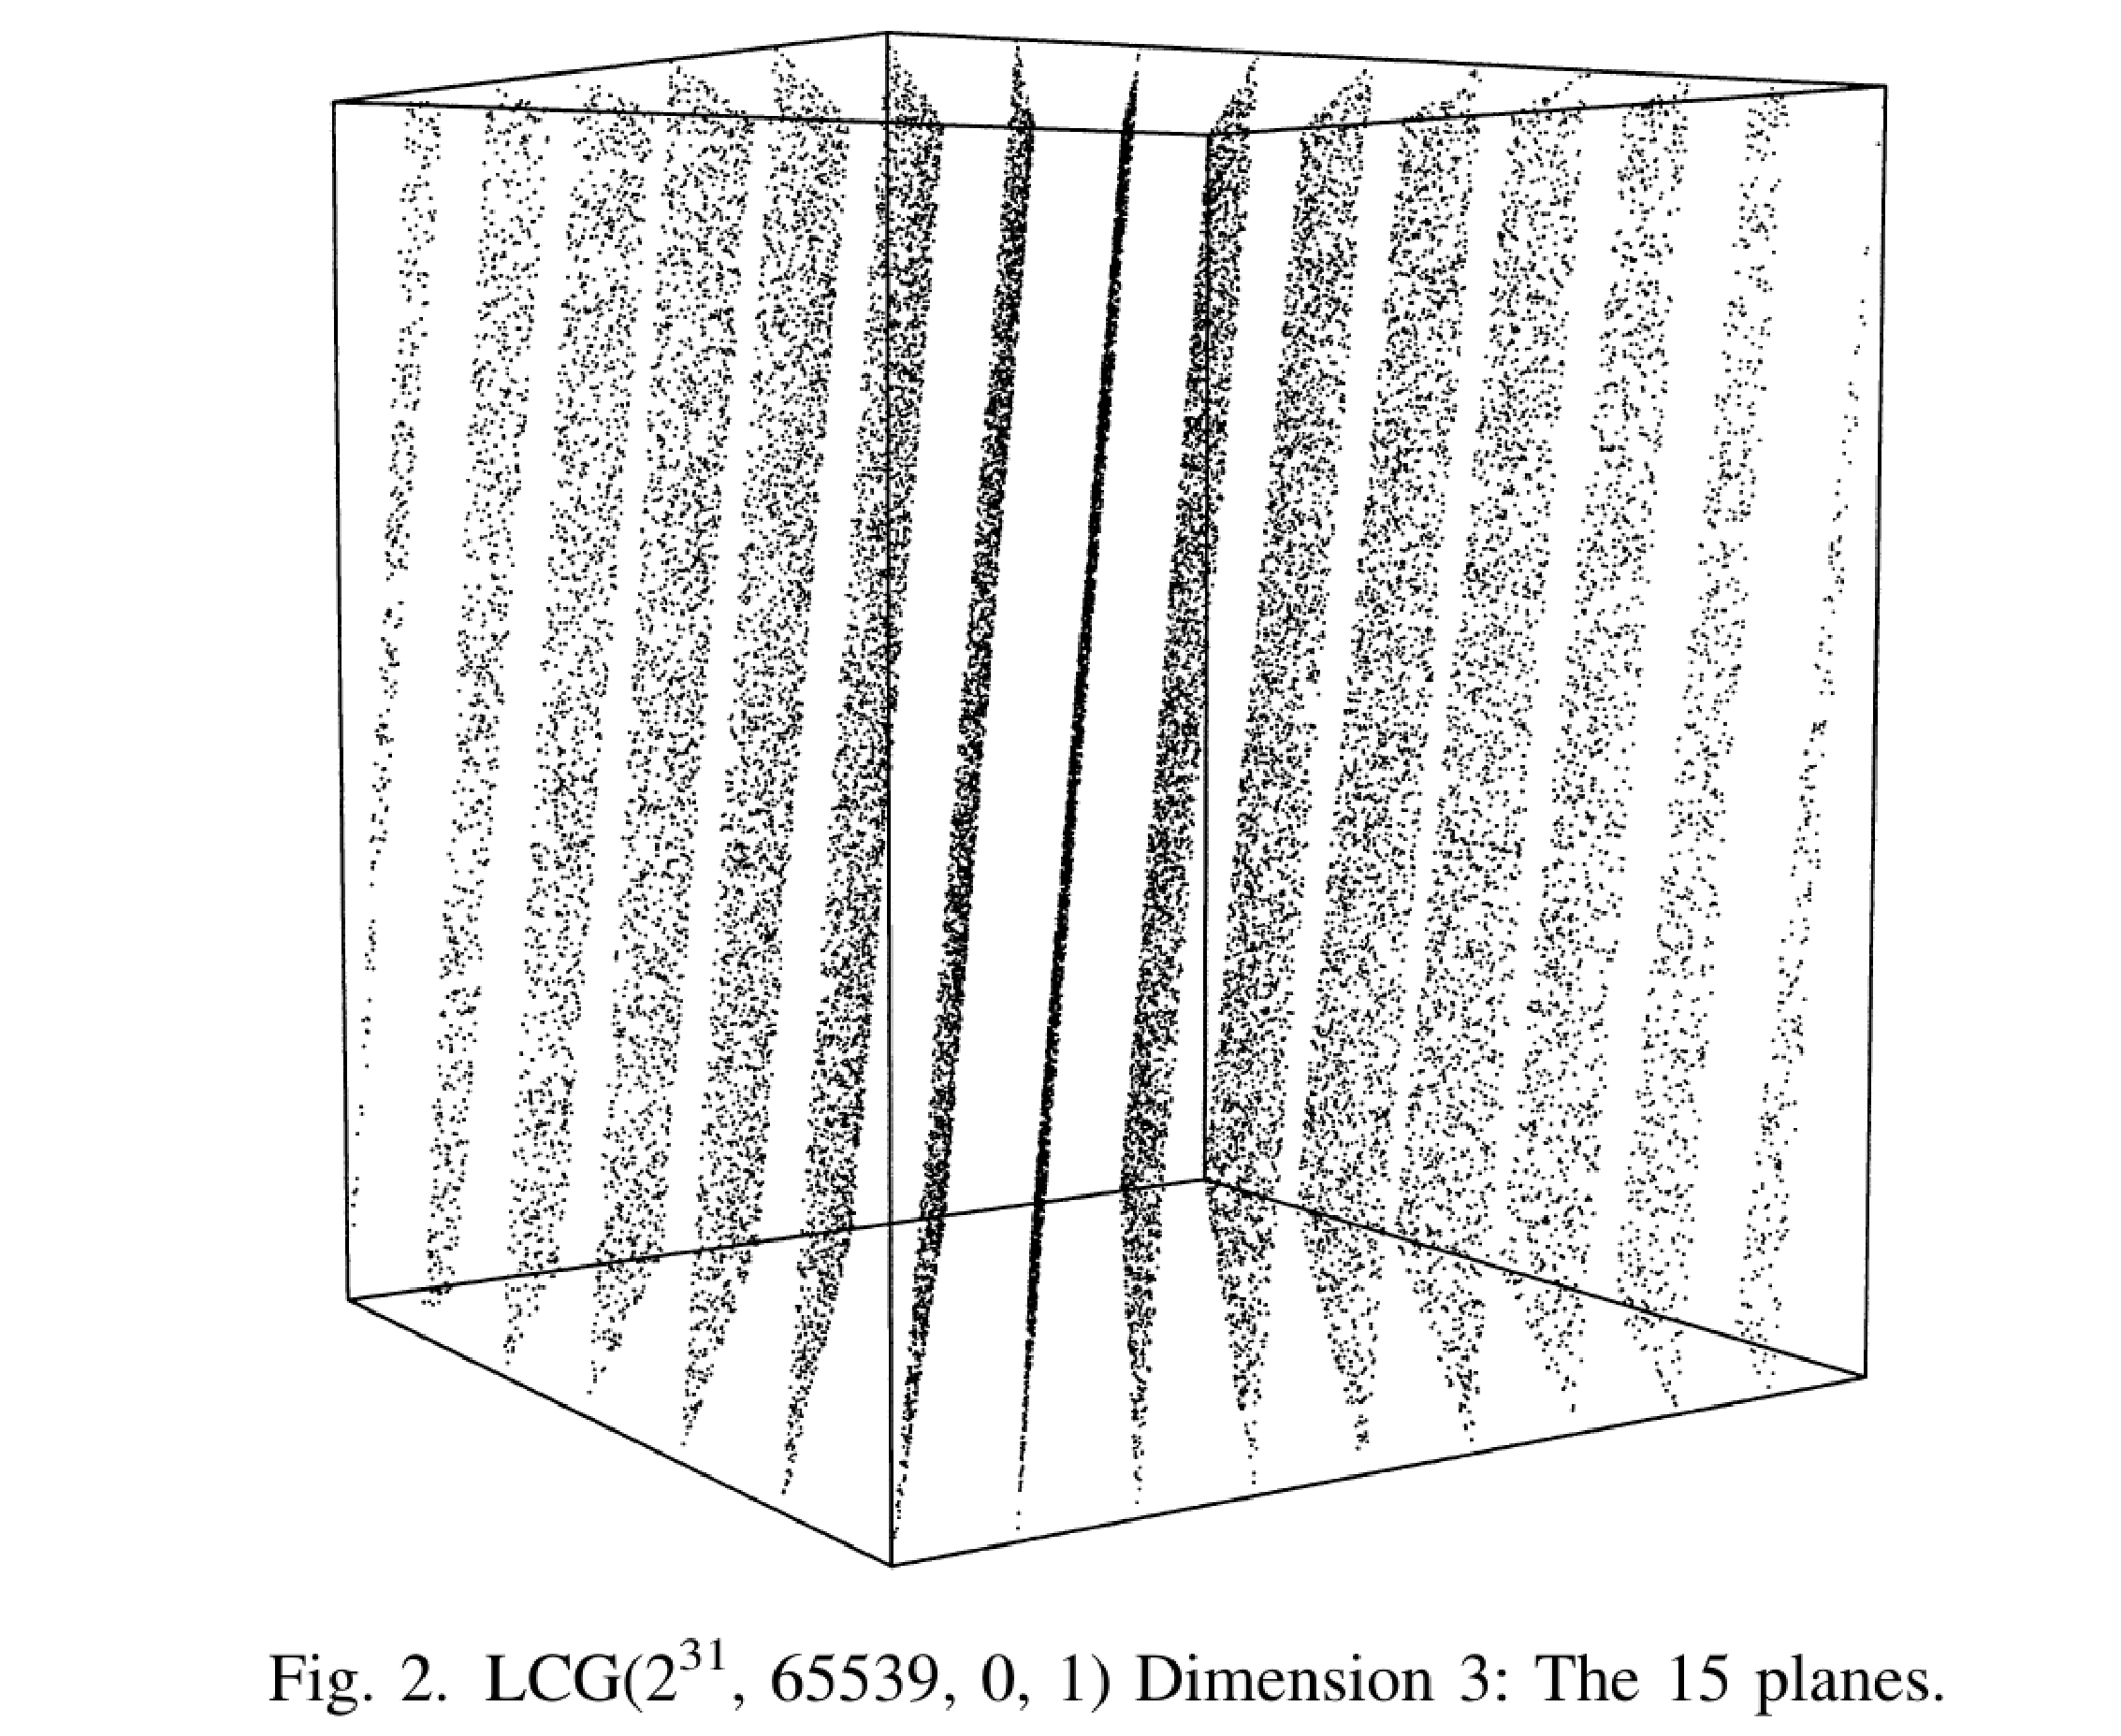
\includegraphics[width=\columnwidth]{figures/random3d.eps}
  }
  {\it\color{pdcolor3}Mathematics and Computers in Simulations 46 (1998) 485-505}
\vfill\null
\end{slide}


%\begin{slide}[toc=Hit-or-miss method]{MC integration (hit-or-miss method)}
\null\vfill

  Lets do the following integration using MC method:
  
  $$\int_0^1 f(x)dx = \int_0^1 \left(\frac{1}{2}x\right) dx = \left.\frac{1}{2}\frac{x^2}{2}\right|_{0}^{1} = \frac{1}{4}$$

  \twocolumn
  {
    \sep
    \begin{itemize}
     \item take a random point from the $[0,1]\times[0,1]$ square
     \item compare it to your $f(x)$
     \item repeat $N$ times
     \item count $n$ points below the function
     \item you results is given by
     $$\int_0^1 f(x)dx = P_{\square} \cdot \frac{n}{N} = \frac{n}{N}$$
    \end{itemize}
  }
  {
    \input{figures/mcExample.tex}
  }
  
\vfill\null
\end{slide}

\begin{emptyslide}{MC integration results}
\null\vfill

  \twocolumn
  {
    
    \includegraphics[width=\columnwidth]{figures/int100.eps}
    \includegraphics[width=\columnwidth]{figures/int1000.eps}
  }
  {
    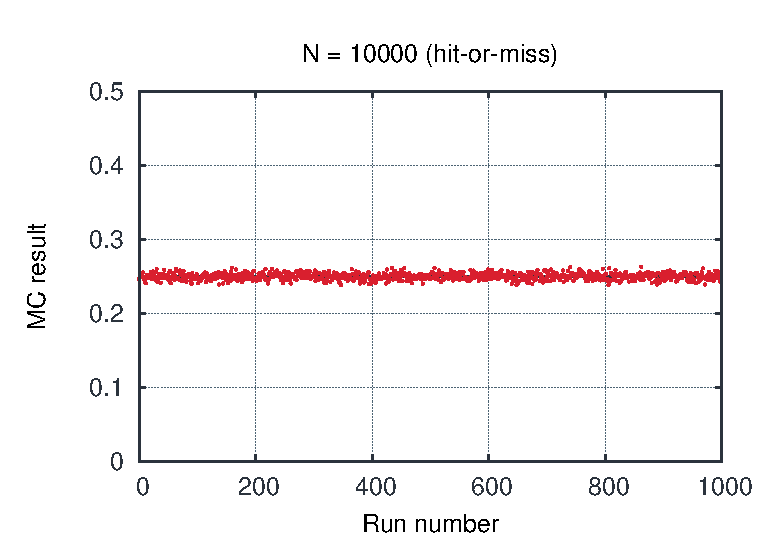
\includegraphics[width=\columnwidth]{figures/int10000.eps}
    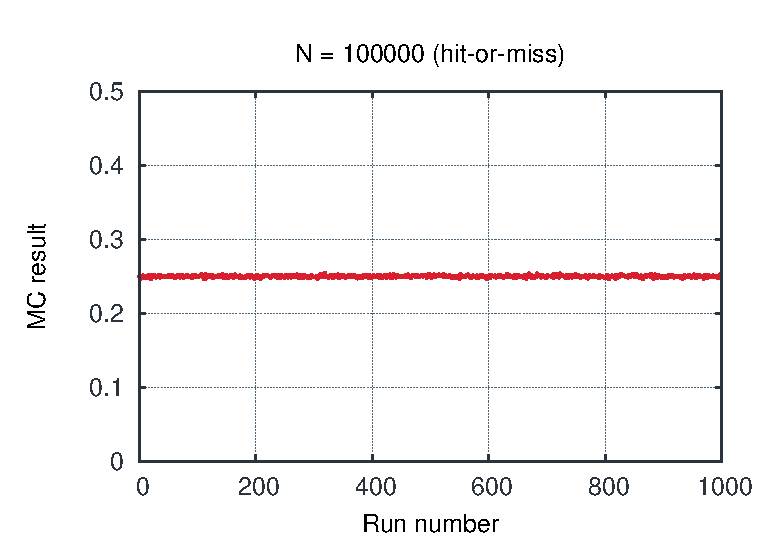
\includegraphics[width=\columnwidth]{figures/int100000.eps}
  }

\vfill\null
\end{emptyslide}


\begin{slide}{Optimization of MC}
\null\vfill

  \twocolumn
  {
    \scalebox{.75}{\input{figures/mcExample.tex}}
  }
  {
    \scalebox{.75}{\input{figures/mcExample2.tex}}
  }

  \begin{itemize}
   \item You want to avoid generating ``red'' points as they do not contribute to your integral
   \item You can choose any rectangle as far as it contains maximum of $f(x)$ in given range
  \end{itemize}

\vfill\null
\end{slide}

\begin{slide}[toc=]{Optimization of MC}
\null\vfill

  \twocolumn
  {
    \begin{itemize}
      \item Lets consider the following function:
  
      $$F(Q^2) = \frac{1}{(1 + Q^2)^2}$$
      {\it\color{pdcolor3} more or less dipole form factor}
      
      \item Integrating this function over $Q^2$ is highly inefficient
      
      \item However, one can integrate by substitution to get better performance, e.g.
      
      $$x = \mbox{log}_{10}(Q^2)$$
      
    \sep{\it\color{pdcolor6}don't forget about Jacobian}

    \end{itemize}

  }
  {
    \usetikzlibrary{calc}

\pgfplotsset{every  tick/.style={pdcolor3,}, minor x tick num=1,}

\begin{tikzpicture}

  \begin{axis}[xlabel = $Q^2$, ylabel = $F(Q^2)$, ylabel near ticks, domain=1:10, scale=0.5, axis lines = left, inner axis line style={>=latex}, ymin = 0, ymax = 0.275, xmin = 1, xmax = 10.5]
    
    \addplot[mark=none, color=pdcolor1, ultra thick] {1 / (1 + x) / (1 + x)};
    \addplot[mark=none, dashed, color=pdcolor3, thick] coordinates {(1,0.25) (10,0.25) (10,0)};

    
    \foreach \x in {1,...,200}
    {
      \pgfmathparse{rnd}
      \pgfmathsetmacro{\a}{9.0*\pgfmathresult + 0.95}
      \pgfmathparse{rnd}
      \pgfmathsetmacro{\b}{0.23*\pgfmathresult + 0.01}
      \pgfmathsetmacro{\c}{\b - 1 / (1 + \a) / (1 + \a)}
      	  
      \ifthenelse{\lengthtest{\c pt > 0.01 pt}}{\addplot[mark=*, mark size = 1pt, color=pdcolor6] coordinates {(\a, \b)};}{}
      \ifthenelse{\lengthtest{\c pt < -0.01 pt}}{\addplot[mark=*, mark size = 1pt, color=pdcolor7] coordinates {(\a, \b)};}{}
    }
    
  \end{axis}

\end{tikzpicture}
    \vspace{-10pt}
    \usetikzlibrary{calc}

\pgfplotsset{every  tick/.style={pdcolor3,}, minor x tick num=1,}

\begin{tikzpicture}

  \begin{axis}[xlabel = {$x = \mbox{log}_{10}(Q^2)$}, ylabel = $F(x)$, ylabel near ticks, domain=-2:1, scale=0.5, axis lines = left, inner axis line style={>=latex}, ymin = 0, ymax = 1.25, xmin = -2, xmax = 1.25]
    
    \addplot[mark=none, color=pdcolor1, ultra thick] {1 / (1 + 10^x) / (1 + 10^x)};
    \addplot[mark=none, dashed, color=pdcolor3, thick] coordinates {(-2,1) (1,1) (1,0)};
    
    \foreach \x in {1,...,200}
    {
      \pgfmathparse{rnd}
      \pgfmathsetmacro{\a}{-2.90*\pgfmathresult + 0.95}
      \pgfmathparse{rnd}
      \pgfmathsetmacro{\b}{0.90*\pgfmathresult + 0.05}
      \pgfmathsetmacro{\d}{-0.175 * (\a + 2) * (\a + 2) + 1}
      \pgfmathsetmacro{\c}{\b - \d}
      	  
      \ifthenelse{\lengthtest{\c pt > 0.1 pt}}{\addplot[mark=*, mark size = 1pt, color=pdcolor6] coordinates {(\a, \b)};}{}
      \ifthenelse{\lengthtest{\c pt < - 0.1 pt}}{\addplot[mark=*, mark size = 1pt, color=pdcolor7] coordinates {(\a, \b)};}{}
    }
    
  \end{axis}

\end{tikzpicture}
    
  }
    
\vfill\null
\end{slide}

\begin{slide}[toc=Crude method]{MC integration (crude method)}
\null\vfill

  Lets do the following integration using MC method once again:
  
  $$\int_0^1 f(x)dx = \int_0^1 \left(\frac{1}{2}x\right) dx = \left.\frac{1}{2}\frac{x^2}{2}\right|_{0}^{1} = \frac{1}{4}$$
  \twocolumn
  {
    \begin{itemize}
      \item One can approximate integral
      \vspace{-5pt}
      $$\int_a^b f(x) dx \approx \frac{b - a}{N}\sum_{i=1}^{N} f(x_i)$$
     
      where $x_i$ is a random number from $[a, b]$
      
      \item It can be shown that crude method is more accurate than hit-or-miss
      
      \item We will skip the math and look at some comparisons
      
    \end{itemize}
  }
  {
    \input{figures/mcExample3.tex}
  }

\vfill\null
\end{slide}

\begin{emptyslide}{Methods comparison}
\null\vfill

  \twocolumn
  {
    \includegraphics[width=\columnwidth]{figures/int100.eps}
    \includegraphics[width=\columnwidth]{figures/int1000.eps}
  }
  {
    \includegraphics[width=\columnwidth]{figures/int2100.eps}
    \includegraphics[width=\columnwidth]{figures/int21000.eps}
  }

\vfill\null
\end{emptyslide}


\begin{slide}[toc=Random from PDF]{Random numbers from probability density function}
\null\vfill

  \twocolumn
  {
    \begin{itemize}
      \item How to generate a random number from probability density function?
      \item Lets consider $f(x) = 3x^2$
      \item Which means that $x = 1$ should be thrown $2$ times more often than $x = \frac{\sqrt{2}}{2}$
    \end{itemize}
  }
  {
    \usetikzlibrary{calc}

\pgfplotsset{every  tick/.style={pdcolor3,}, minor x tick num=1,}

\begin{tikzpicture}

  \begin{axis}[xlabel = {$x$}, ylabel = {$y$}, ylabel near ticks, domain=0:1, scale=0.5, axis lines = left, inner axis line style={>=latex}, ymin = 0, ymax = 3.25, xmin = 0, xmax = 1.1]
    
    \addplot[mark=none, color=pdcolor1, ultra thick] {3*x^2};
    \addplot[mark=*, mark size = 2pt, color=pdcolor6] coordinates {(0.75, 1.6875)};

    \addplot[mark=none, dashed, color=pdcolor3, thick] coordinates {(0, 1.6875) (0.75, 1.6875) (0.75, 0)};
    
%    \node[right] at (axis cs:  0.75, 1.6875) {$(\frac{3}{4}, \frac{27}{16})$};
    
    %\addplot table[x = x, y = y, col sep = space] {data/forceDist.dat};
    
  \end{axis}

\end{tikzpicture}

  }

\vfill\null
\end{slide}

\begin{slide}[toc=CDF]{Cumulative distribution function}
\null\vfill

  \begin{itemize}
    
    \item Cumulative distribution function of a random variable $X$:
    
    $$F(x) = P (X \leq x)$$
    
    \sep
    {\it\color{pdcolor3} Note: $0 \leq F(x) \leq 1$ for all $x$}
        
    \item Discrete random variable $X$:
    
    $$F (x) = \sum\limits_{x_i \leq x} f (x_i)$$

    where $f$ is probability mass function (PMF)
    
    \item Continuous random variable $X$:
    
    $$F (x) = \int\limits_{-\infty}^{x} f (t) dt$$ 
        
    where $f$ is probability density function (PDF)

    \end{itemize}

\vfill\null
\end{slide}

\begin{slide}[toc=CDF discrete]{Cumulative distribution function - discrete example}
\null\vfill

  \begin{itemize}
    
    \item Probability mass function $f(x) = 3x^2$
    \item[] with discrete random variables $X$ is $\{\sqrt{\frac{1}{30}}, \sqrt{\frac{2}{30}}, \sqrt{\frac{3}{30}}, \sqrt{\frac{4}{30}},\}$
    \item CDF is given by:
    
  \end{itemize}
  
  \twocolumn
  {
  $$F (x) = \begin{cases}
	      \frac{1}{10}  & \mbox{if~~~} x \leq \sqrt{\frac{1}{30}} \\
	      \frac{3}{10}  & \mbox{if~~~} x \leq \sqrt{\frac{2}{30}} \\
	      \frac{6}{10}  & \mbox{if~~~} x \leq \sqrt{\frac{3}{30}} \\
	      \frac{10}{10} & \mbox{if~~~} x \leq \sqrt{\frac{4}{30}} 
	    \end{cases}
  $$
  }
  {
    \input{figures/discreteCDF.tex}
  }
  \vspace{-10pt}
  \begin{itemize}
  
    \item With $P = 1$ the random number is less or equal to $\sqrt{\frac{4}{30}}$, with $P = 0.6$ the random number is less or equal $\sqrt{\frac{3}{30}}$ ...
    
  \end{itemize}

\vfill\null
\end{slide}

\begin{slide}[toc=]{Cumulative distribution function - discrete example}
\null\vfill
  
 \begin{itemize}
  \item To generate a random number from $X$ according to $3x^2$:
  \begin{itemize}
    \item generate a random number $u$ from $[0, 1]$
    \item if $u \leq 0.1$: $x = \sqrt{\frac{1}{30}}$
    \item else if $u \leq 0.3$: $x = \sqrt{\frac{2}{30}}$ ...
  \end{itemize}
  \item Results for $N = 10000$:
 \end{itemize}

 \begin{center}
 \begin{tabular}{c|c|c|c}
$x$ & $n$ & $n/N$ & $f(x)$ \\ \hline 
$\sqrt{\frac{1}{30}}$ &  989  & 0.0989 & 0.1 \\
$\sqrt{\frac{2}{30}}$ & 1959 & 0.1959 & 0.2 \\
$\sqrt{\frac{3}{30}}$ & 2949 & 0.2949 & 0.3 \\
$\sqrt{\frac{4}{30}}$ & 4103 & 0.4103 & 0.4 \\
 \end{tabular}
 \end{center}
 
\vfill\null
\end{slide}

\begin{slide}[toc=CDF continuous]{Cumulative distribution function - continuous example}
\null\vfill

  \begin{itemize}
    
    \item Probability density function $f(x) = 3x^2$
    \item[] with continuous random variables $X$ range $[0, 1]$
    \item CDF is given by:
    
  \end{itemize}
  
  \twocolumn
  {
    \begin{eqnarray*}
      F (x) & = & \int\limits_0^x f(t) dt \\
            & = & \int\limits_0^x 3t^2 dt \\
            & = & \left.t^3\right|_0^x = x^3
    \end{eqnarray*}
  }
  {
    \input{figures/continuousCDF.tex}
  }
  
  \begin{itemize}
  
    \item Blue area gives the probability that $x \leq 0.75$
    
  \end{itemize}

\vfill\null
\end{slide}

\begin{slide}[toc=]{Cumulative distribution function - continuous example}
\null\vfill

 \begin{itemize}
  \item To generate a random number from $X$ according to $3x^2$:
  \begin{itemize}
    \item generate a random number $u$ from $[0, 1]$
    \item find $x$ for which $F (x) = u$, i.e. $x = F^{-1}(u)$
    \item $x$ is your guy
  \end{itemize}
  \item Results for $N = 10000$:
 \end{itemize}
  \sep
 \twocolumn
 {
  \input{figures/cCDFexample.tex}
 }
 {
  \sep\sep\sep
  Unfortunately, usually $F^{-1}$ is unknown, which makes this method pretty useless (at least directly).
 }
\vfill\null
\end{slide}


\begin{slide}[toc=Acceptance-rejection]{Acceptance-rejection method}
\null\vfill

  \twocolumn
  {
    \begin{itemize}
      \item Lets consider
      $$f(x) = A \cdot x^3 \cdot e^{-x^2}$$
      with $x \in [0, 1]$, $A = \frac{2e}{e-2}$ 
      \item CDF is given by
      $$F(x) = \frac{N}{2}(x^2 - 1)e^{-x^2}$$
    \end{itemize}
  }
  {
    \input{figures/ar1.tex}
  }
  
  \begin{itemize}
    \item Since, we do not know $F^{-1}$ we have to find another way to generate $x$ from $f(x)$ distribution
    \item We will use acceptance-rejection method (do you remember MC integration via hit-or-miss?)
  \end{itemize}

\vfill\null
\end{slide}

\begin{slide}[toc=]{Acceptance-rejection method}
\null\vfill

  \twocolumn
  {
    \begin{itemize}
      \item Evaluate $f_{max} \geq \mbox{max}(f)$
      \item[] {\it\color{pdcolor3}Note: $f_{max} > \mbox{max}(f)$ will affect performance, but the result will be still correct}
      \item Generate random $x$
      \item Accept $x$ with $P = \frac{f(x)}{f_{max}}$
      \begin{itemize}
	\item generate a random $u$ from $[0, f_{max}]$
	\item accept if $u < f(x)$
      \end{itemize}
      \item The plot on the right shows the results for $N = 10^5$
    \end{itemize}
  }
  {
    \input{figures/ar2.tex}
    \input{figures/ar3.tex}
  }

\vfill\null
\end{slide}

\begin{slide}[toc=]{Acceptance-rejection method - optimization}
\null\vfill

  \twocolumn
  {
    \begin{itemize}
      \item The area under the plot of $f(x)$ is $\sim 0.13$
      \item The total area is $0.4$
      \item Thus, only about $30\%$ of points gives contribution to the final distribution
      \item One can find $g(x)$ for which CDF method is possible and which encapsulates $f(x)$ in given range and generate $x$ according to $g(x)$
      \item For $g(x) = 0.4 x$ the total area is $0.2$, so we speed up twice
    \end{itemize}
  }
  {
    \input{figures/ar4.tex}
    \input{figures/ar5.tex}
  }

\vfill\null
\end{slide}


\begin{slide}[toc=]{Acceptance-rejection method - optimization}
\null\vfill

  \begin{itemize}
    \item Cumulative distribution function for $g(x) = 2x$
    
    $$G(x) = \int_0^x g(t)dt = x^2 \Rightarrow G^{-1}(x) = \sqrt{x}$$
    
    {\it\color{pdcolor3}Note: PDF must be normalized to 1 for CDF}
    
    \item Generate random number $u \in [0, 1]$
    \item Calculate your $x = G^{-1}(u)$
    \item Accept $x$ with probability $P = f(x) / g(x)$
    \item[] {\it\color{pdcolor3}instead of using constant $f_{max}$ we are using $f_{max}(x) \equiv g(x)$}
    
  \end{itemize}

\vfill\null
\end{slide}




\section{Quasi-elastic scattering}

\begin{wideslide}[toc=QEL on free N]{Quasi-elastic scattering on a free nucleon}
\null\vfill

  \myBox{Llewellyn-Smith formula}
  
  $$\frac{d\sigma}{dQ^2} {{\nu_l + n \rightarrow l^- + p}\choose{\bar\nu_l + p \rightarrow l^+ + n}} = \frac{M^2G_F^2\cos\theta_C}{8\pi E_\nu^2}\left[A(Q^2) \mp B(Q^2)\frac{(s - u)}{M^2} + C(Q^2)\frac{(s - u)^2}{M^4}\right]$$
  
  \myBox{Notation}
  
  \begin{itemize}
    \item Constants: $M$ - nucleon mass, $G_F$ - Fermi constant, $\theta_C$ - Cabibbo angle,
    \item $Q^2 = -q^2 = - (k - k')^2 = - (p' - p)^2$ - four-momentum squared, where $k$, $k'$, $p$, $p'$ are four-momenta of initial and final lepton, initial and final nucleon
    \item $E_\nu$ - neutrino energy
    \item $s = (k + k')^2$ and $u = (k - p')^2$ - Mandelstam variables
  \end{itemize}

  
\vfill\null
\end{wideslide}

\begin{wideslide}[toc=]{Quasi-elastic scattering on a free nucleon}
\null\vfill

  \myBox{Llewellyn-Smith formula}
  
  $$\frac{d\sigma}{dQ^2} {{\nu_l + n \rightarrow l^- + p}\choose{\bar\nu_l + p \rightarrow l^+ + n}} = \frac{M^2G_F^2\cos\theta_C}{8\pi E_\nu^2}\left[A(Q^2) \mp B(Q^2)\frac{(s - u)}{M^2} + C(Q^2)\frac{(s - u)^2}{M^4}\right]$$
  
  \myBox{Lets integrate it}
  
  \begin{itemize}
    \item Having $k$ and $p$, generate $k'$ and $p'$ (usually in center of mass system) from whole available phase space
    \item Calculate $Q^2$ and $s - u$ based on kinematics
    \item Calculate cross section
    \item Repeat $N$ times and the result is given by: 
    
    \vspace{-32pt}$$\hspace*{150pt}\sigma_{total} = \frac{Q^2_{max}}{N} \sum\limits_{i = 1}^N \sigma (Q_i^2)$$
    
  \end{itemize}

  
\vfill\null
\end{wideslide}


\end{document}
